\chapter{Detecting Features and Patterns}

\section{Image edges and image derivatives}

\textbf{Goal:} Identify sudden changes in an image. Most semantic shape information is within edges.

\textbf{Causes for edges:} Reflection changes (appearance information and texture), Depth discontinuity, Shadows, Changes in surface orientation (shape).

Plotted using itensity as height, edges appear as "cliffs" $\rightarrow$ Low-level edges characterized by \textbf{gradient magnitude}.

\textbf{Problems of edge detection:} Intensity changes are often not linked to the actual object contours, hence we get a lot of unuseful information. Causes can be: Strong intensity changes (texture, shadows), No intensity change at boundary (background texture similar, too dark,...).

Human edge detection: High-level (object-level), completion of invisible contours, shadow removal, ... .

\textbf{Concentrating on gradient-based edge detection}!

\subsection{Image derivatives}

\textbf{Continuous derivative:} $\partial_x f(x,y) = \lim_{\epsilon \rightarrow \infty} \dfrac{f(x + \epsilon, y) -f(x,y)}{\epsilon}$

\textbf{Discrete versions:}

\begin{description}
    \item[Forward diff.] $(\partial_x f)_{i,j}) = \dfrac{f(i+1,j) - f(i,j)}{h_x}$
    \item[Backward diff.] $(\partial_x f)_{i,j}) = \dfrac{f(i,j) - f(i-1,j)}{h_x}$
    \item[Central diff.] $(\partial_x f)_{i,j}) = \dfrac{f(i+1,j) - f(i-1,j)}{2h_x}$
\end{description}

With (convolution) kernels $[1,-1,0], [0,1,-1], [1/2, 0, -1/2]$. The same holds for derivative in y-direction, only with transposed vectors, i.e., column vector.

\textbf{Gradient:} The gradient $\nabla f = (\partial_x f, \partial_y f)$ is the derivative in both directions and can be interpreted as vector-valued image with $n=m=2$, the gradient points strongest changes in each direction.

\textbf{Gradient magnitude:} $||\nabla f|| = \sqrt{(\partial_x f)^2 + (\partial_y f)^2}$ is the length of the vector. \textbf{Larger magnitude, stronger changes}.

Problems with noise and derivatives:\textbf{ High frequency content is amplified, since they are strong changes!} Hence, first smooth signal (image) then apply derivative.

\subsection{Convolution and Derivatives}

Smoothing needs convolving, which is needed when noisy image derivatives are to be calculated.

\textbf{Continuous Conv.:} $(f*g)(x) = \int_{\mathbb{R}^N} f(x-u)g(u) du$, same as discrete only with integral.

\textbf{Derivative theorem for cont. conv.:} $\partial_i (f*g) = (\partial_i f)*g = f * (\partial_i g)$, more efficient to only have to calculate one derivative. Needs some conditions on $f$ and $g$!

When met, a kernel derivative can be precomputed and applied using convolution (for instance Gaussian on LS 2.20).

\textbf{Advantages:} Precomputation (Efficiency); Filter function is known, then coefficients can be precomuted analytically!

\textbf{Example:} Derivative using gaussian derivative filter: 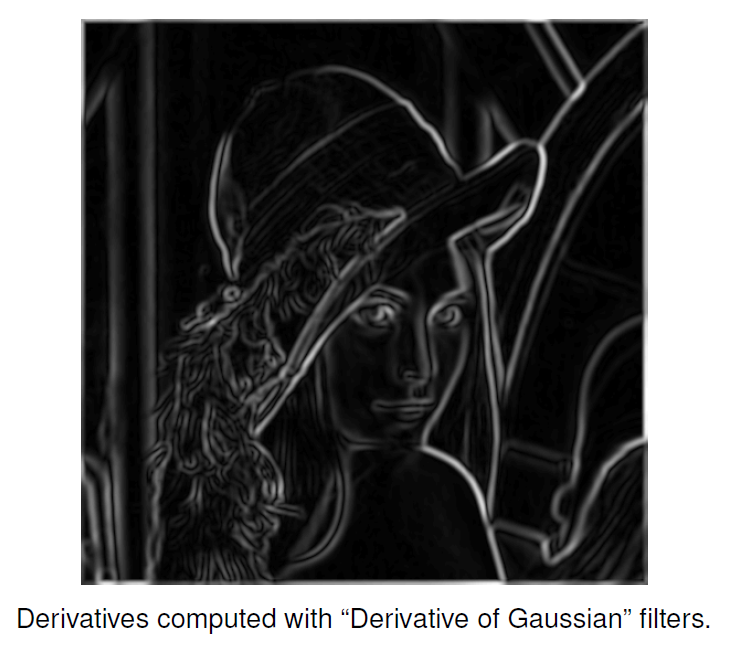
\includegraphics[width=.3\textwidth]{images/chap3/der_gauss}

\subsection{Canny Edge Detection}

How to find the edge when we have the derivative image?

\textbf{Non-maxima suppression idea:} Keep pixels that are on local maxima along the gradient direction (interpolation).

\textbf{Process:}

\begin{itemize}
    \item Filter with derivative of gaussian at scale $\sigma$
    \item Find magnitude and oritentation of gradient
    \item Non-maxima suppression!
    \item Linking, thresholding, two thresholds \textbf{low and max}, low starts edges and high continues them.
\end{itemize}

\subsection{Scale-space}

Applying gaussian filter with incrementing $\sigma$ removes "detail": \textbf{Scale-space}

\begin{itemize}
    \item Edges may shift with increasing $\sigma$
    \item Edges may merge!
    \item Edges may not split into two
    \item Multiple ways to calculate scale-spaces, \textbf{gaussian} is the "canonical" one
\end{itemize}

\section{Feature detection: the fundamentals}

\textbf{Steps for matching:}

\begin{itemize}
    \item \textbf{Detection}, identify points
    \item \textbf{Description}, extract information (feature vector)
    \item \textbf{Match}, correspondences between descriptors
\end{itemize}

\textbf{Goals for detectors:}

\begin{itemize}
    \item \textbf{Locality}, features local, robust to occlusion and clutter
    \item \textbf{Quantity}, many for one image
    \item \textbf{Distinctiveness}, differentiate large amount of objects
    \item \textbf{Efficiency}, real-time scalability
    \item \textbf{Geometric invariance}, translation, rotation, scale!!
    \item \textbf{Photometric invariance}, intensity, brighteness, contrast, exposure
\end{itemize}

\subsection{Good features}
\textbf{What points to choose?}: Large contrast changes, gradients in two different image orientations (corners)..

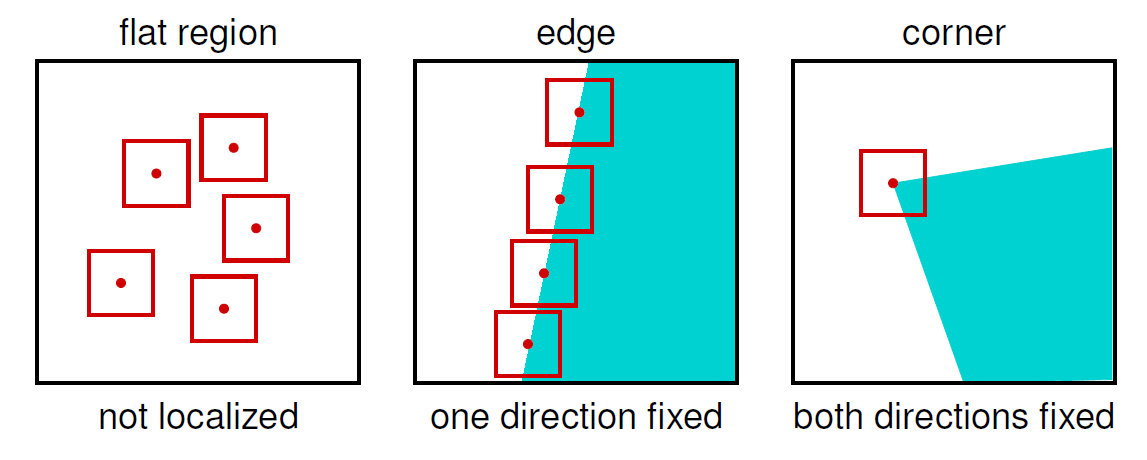
\includegraphics[width=.7\textwidth]{images/chap3/good_feature}

The image shows that only corners have unique regions, even on edges we have multiple similar patches.

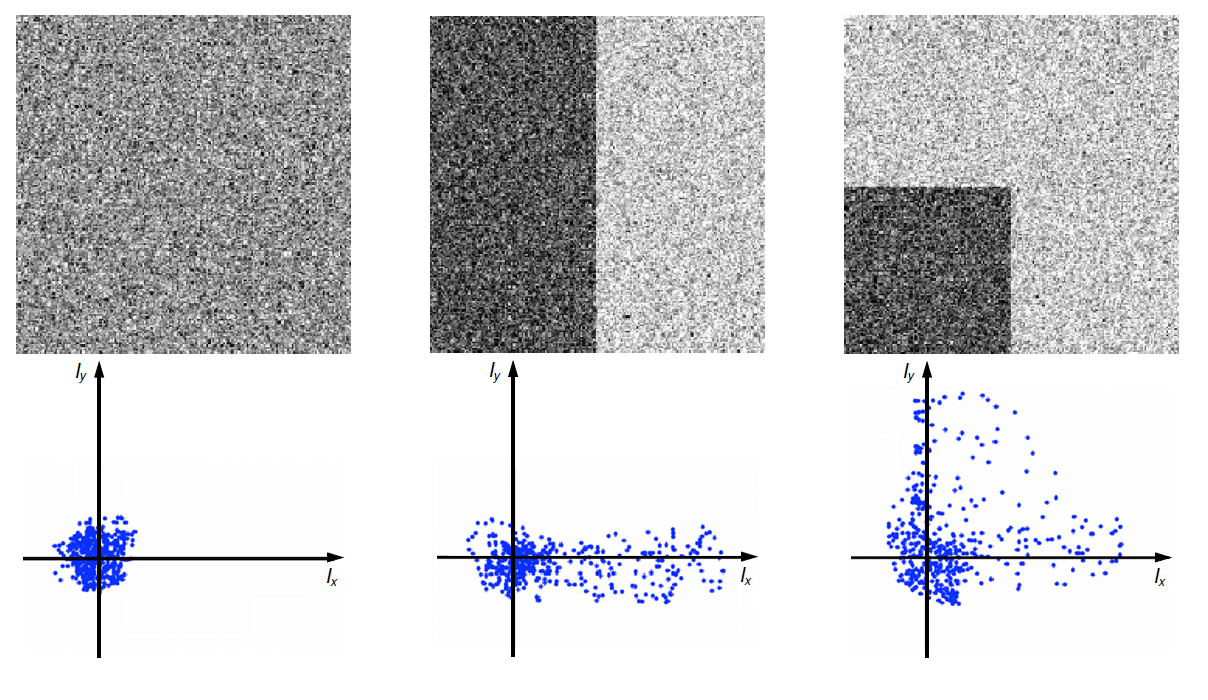
\includegraphics[width=.7\textwidth]{images/chap3/feature_dist}

This image shows the distribution of data. When we have a corner, we have points in both directions.

\subsection{Maths: SVD}

A matrix $A \in \mathbb{R}^{m\times n}$ can be factorized in the form of $A = U \Sigma V^T$, where

\begin{itemize}
    \item $U \in \mathbb{R}^{m\times m}$ is orthogonal, $UU^T = U^T U = I_m$
    \item $V \in \mathbb{R}^{n \times n}$ is orthogonal 
    \item $\Sigma \in \mathbb{R}^{m\times n}$ is diagonal, sorted non-neg. real numbers $\sigma_1 \geq \sigma_2 \geq ... \geq 0$ and are called singular values of A.
\end{itemize}

\textbf{Singular values} are uniquely determined, $U,V$ are not. $AV = \Sigma U$ shows that, $A$ maps $V$ to $U$ scaled by $\Sigma$.
\begin{itemize}
\item \textbf{Rank of matrix:} Number of non-zero singular values
\item \textbf{Range of $A$:} Spanned by columns of $U$ where singular values non-zero (i.e. rank)
\item Columns of $V$ are eigenvectors of $A^T A$
\item Columns of $U$ are eigenvectors of $AA^T$
\item Eigenvalues of $A^T A$ and $AA^T$ are squared singular values.
\item Eigenvalues only positive or zero.
\end{itemize}

\textbf{Applications:}

\begin{itemize}
    \item Can solve problems of type $argmin_{|x| = 1} ||A_x||$
    \item PCA
    \item Linear least square for homography estimation  $argmin_{|x| = 1} ||A_x - b||^2$
\end{itemize}

\textbf{Interpretation:}

\begin{itemize}
    \item Columns of $V$ give new basis for vector space $\mathbb{R}^n$
    \item Face data: Space of possible images of faces
    \item New basis vectors are chosen to capture most important aspects of data in descending order of importance
    \item Importance corresponds to magnitude of singular value
\end{itemize}

\textbf{PCA:} Intuition of SVD is formalized in PCA. Goal is to characterize probability dists. of variables, for example to find the directions with greatest variance.

\textbf{Joint probability distributions terminology}:

\begin{itemize}
    \item Random Variables $X_j, j=1,..,n$, two variables we call it \textbf{bivariate}
    \item \textbf{Joint distribution}, $P(X_j=x_j \forall j)$ in the image, samples inside green ellipse
    \item Marginal distributions, $P(X_j = x_j)$, i.e., $P(X=x)(blue), P(Y=y)(red)$ in the image.
    \item $X_j, X_k$ independent iff  $P(X_j=x_j, X_k=x_k) = P(X_j = x_j)P(X_k=x_k)$
\end{itemize}

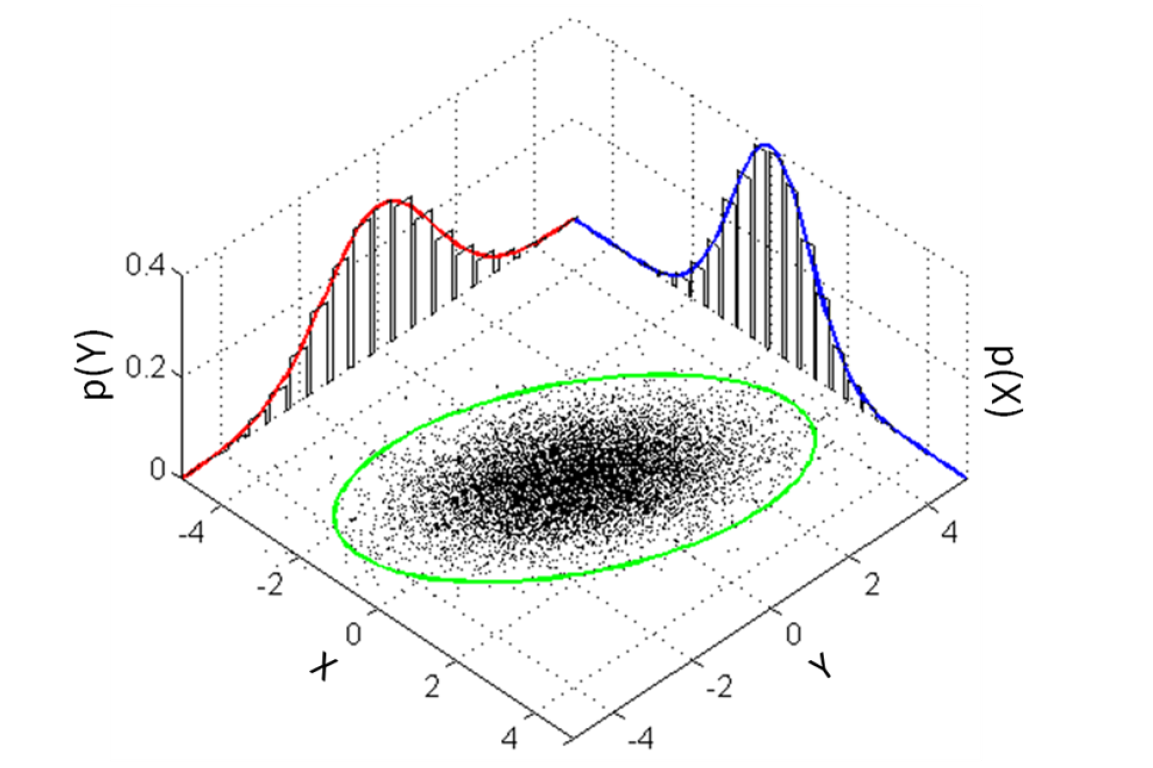
\includegraphics[width=.7\textwidth]{images/chap3/joint_dist}

\textbf{Expected sample value:}  $E(Z) = \sum p_iz_i$, weighted average over all measurements for $Z$.

\textbf{Sample variance:} $Var(Z) = \sum p_i(Z_i - E(Z))^2$, expected squared deviation from the expectation value.

\textbf{Sample standard deviation:} Squareroot of variance is $\sigma(Z)$

\textbf{Covariance of two random Variables X,Y:} $cov(X,Y) = \sum p_i(x_i - E(X))(y_i - E(Y))$.

\textit{Assuming we have centered measurements}, i.e. $E(Z_i) = 0$ for all $Z_i$. Then the covariance is $cov(X_j,X_k) = \sum p_i x_{ji} x_{ki}$.

\textbf{Covariance matrix:} Defined as $n\times n$ matrix for $n$ random variables:

$C(X) := (cov(X_j,X_k))_{j,k=1,\dots,n}$ and properties are: \textbf{Symmetric, Diagonal is Variances, positive semi-definite}. If measurements are row vectors of large matrix $M \in \mathbb{R}^{m\times n}$ and i-th row is multiplied by $\sqrt{p_i}$, we have $C(X) = M^T M$.

\textbf{Covariance Matrix and SVD}

If $M = U \Sigma V^T$, measurements transformed by $V$, we get $M' = MV = U\Sigma$ with cov. $C' = \Sigma^T U^T U \Sigma = \Sigma^2$, i.e., cov. matrix can be made diagonal using orthogonal tranformation! (Eigenvectors of old cov. matrix are mapped to unit vectors). The standard deviations are equal to the singular values.

\textbf{Ellipses}: Two random variables decorrelated. Ellipse given as: 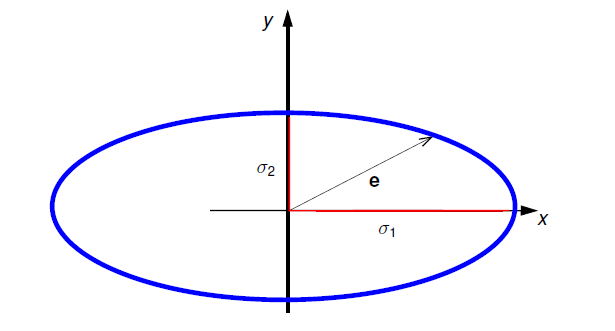
\includegraphics[width=.3\textwidth]{images/chap3/ellipse}

\textbf{Interpretation:} Radius $e = (\sin(\Phi),\cos(\Phi))^T$ is $\sqrt{\sigma_1^2e_1^2+\sigma_2^2e_2^2} = \sqrt{e_1^2 var(X) + e_2^2 var(Y)} = \sqrt{var(e_1X+e_2Y)}$, i.e., radius yields standard deviation projected onto the direction (denoted by $\Phi$).

\textbf{Summary of PCA}

\begin{itemize}
    \item Closely related to SVD
    \item Use to decorrelate data
    \item Dimensions with larger singular values have higher variance, more meaningful
    \item Useful for high-dimensional data analysis, find most meaninungful lower-dimensional representation
    \item Application for gradient measurements around a pixel to analyze local orientations in images
\end{itemize}

\subsection{Structure Tensor}

Gaussian kernel $G_\sigma$, derivative is with scale $\sigma$ is $\partial_x^\sigma = \partial_x * G_\sigma$, for images $f = (f_{i,j})$ we write the partial der. at scale $\sigma$ as $f_x^\sigma, f_y^\sigma$.

\textbf{ST as gradient statistics:} Sample gradient scale $\sigma$ of window for pixel. Interested in local structure, assign weight depending on distance to pixel (gaussian distribution).

Consider gradient to be distributed as \textbf{joint distribution} of partial derivatives $f_x^\sigma, f_y^\sigma$. The distribution around the pixel (i,j) is characterized by the cov. matrix:

$$C(\nabla^\sigma f) = \left[
\begin{matrix}
cov(f_x^\sigma , f_x^\sigma) & cov(f_x^\sigma , f_y^\sigma) \\
cov(f_y^\sigma , f_x^\sigma) & cov(f_y^\sigma , f_y^\sigma)
\end{matrix}\right] = \left[
\begin{matrix}
E(f_x^\sigma f_x^\sigma) & E(f_x^\sigma f_y^\sigma) \\
E(f_y^\sigma f_x^\sigma) & E(f_y^\sigma f_y^\sigma)
\end{matrix}\right]$$

Expanding the formulas, gives the definition of the !\textbf{structure tensor}!, which is
$$\tau = \left[
\begin{matrix}
G_\tau * (f_x^\sigma)^2 & G_\tau * (f_x^\sigma f_y^\sigma) \\
G_\tau * (f_x^\sigma f_y^\sigma) & G_\tau * (f_y^\sigma)^2
\end{matrix}\right] = G_\tau * \left[
\begin{matrix}
 (f_x^\sigma)^2 & (f_x^\sigma f_y^\sigma) \\
(f_x^\sigma f_y^\sigma) & (f_y^\sigma)^2
\end{matrix}\right]$$

a grayscale image whose values are $2\times 2$ matrices. Two parameters are necessary, $\sigma > 0$ is the inner scale for the derivatives and $\tau > 0$ the outer scale parameter which determines the size of the window on which the derivative information is sampled on. Example: \\
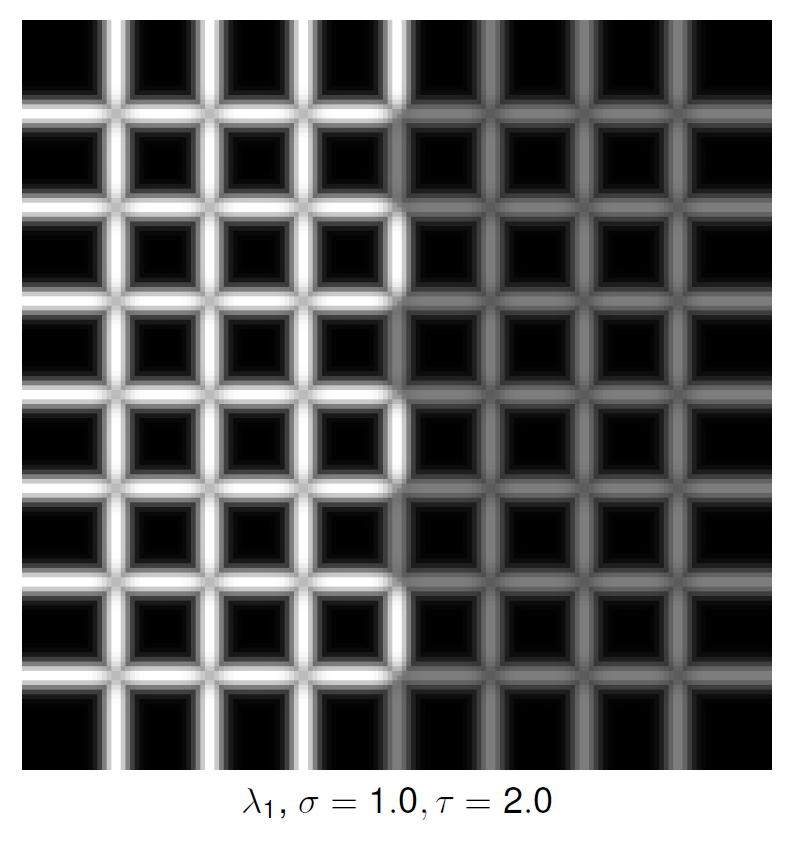
\includegraphics[width=.5\textwidth]{images/chap3/st_ex}

for a checkerboard image and $\lambda_1$ being the first eigenvalue (biggest as well). For $\lambda_2$ boxes can be seen in the example on LS 2.74.

\textbf{Properties based on eigenvalues:}

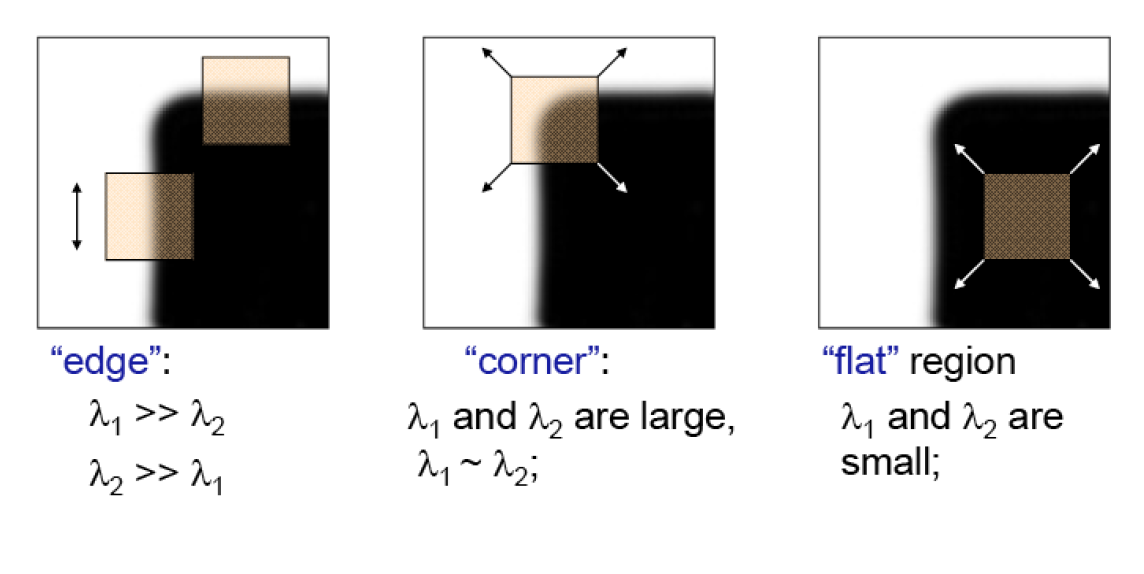
\includegraphics[width=.6\textwidth]{images/chap3/st_props}, i.e. edges are denoted s.t. one of the eigenvalues is much larger, for corners both are large and flat regions both are small. 

\textbf{Cornerness response function:} $\lambda_1 \geq \lambda_2$, multiple functions exist to tell if a point looks like a corner: 

\begin{itemize}
    \item Shi and Tomasi, 1994: $\lambda_2$ smaller is used
    \item Harrise 1988, Foerstner 1986: using $\det(\tau) - \mathcal{K} trace(\tau)^2 = \lambda_1 \lambda_2 - \mathcal{K}(\lambda_1+\lambda_2)^2$
\end{itemize}

Corners are found when a threshold is exceeded and a local maximum is reached.

\section{Pattern matching}

\textbf{Patch comparison:} SSD - sum of squared diffs.: $$E_{SSD}(f,g) = \sum_i^W\sum_j^H (f(i,j)-g(i,j))^2$$, W being the width and H the height of the patch. Example of paramentrization:

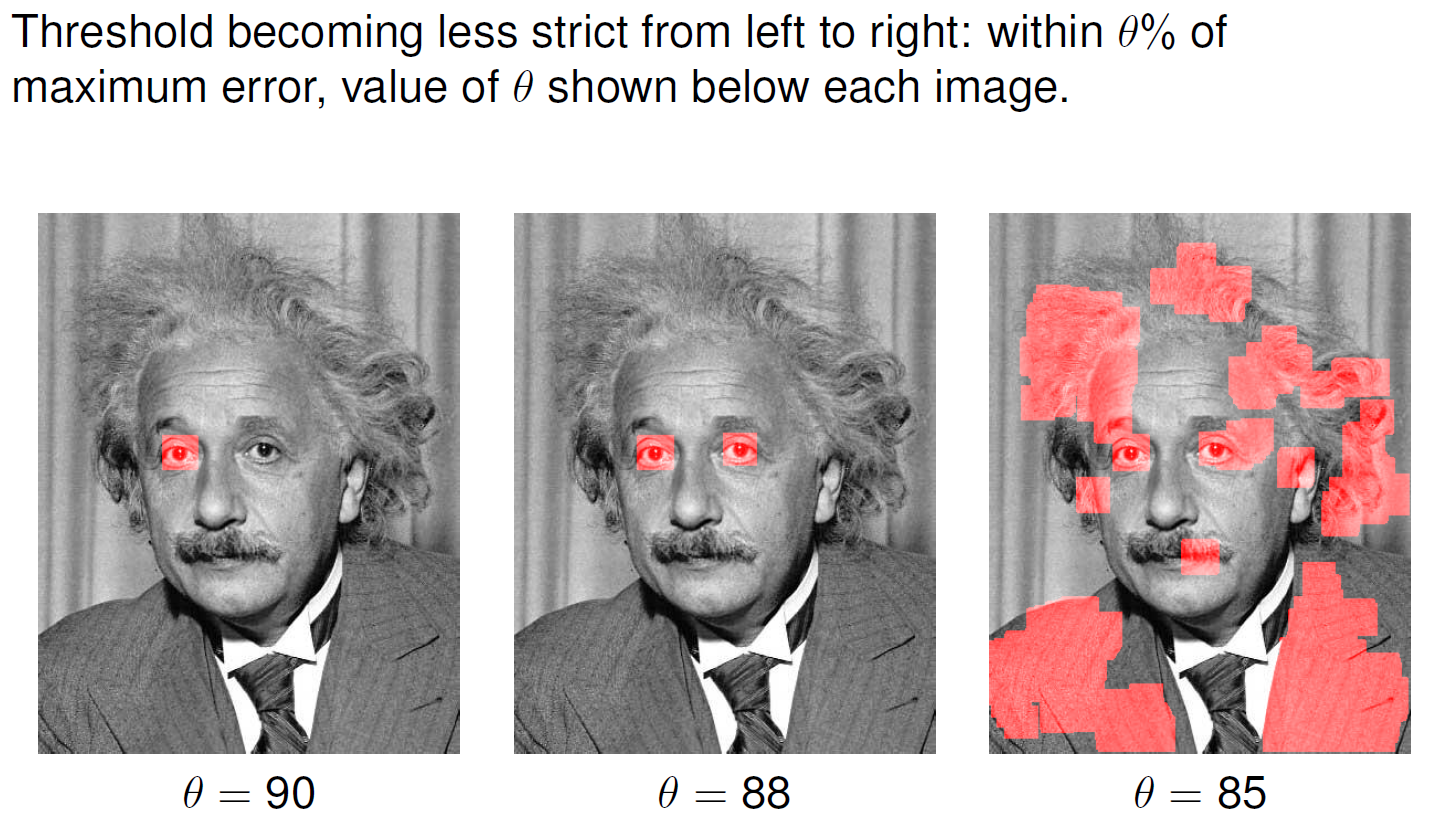
\includegraphics[width=.6\textwidth]{images/chap3/SSD_thresh}

\textbf{Properties as patch comparison metric:}
\begin{tabular}{lr}
    Fast & yes \\
    \hline    
    Invariant to translation & yes \\
    Invariant to rotation & no \\
    Invariant to scaling & no \\
    \hline
    invariant to contrast/brightness changes & No
\end{tabular}

\textbf{Better approach? NCC!}: Given a patch W,H on f,g the \textbf{Normalized Cross-Correlation} distance is defined as $$E_{NCC}(f,g) = \dfrac{cov(f,g)}{\sigma(f)\sigma(g)}$$, range within [-1,1], larger the better.

\textbf{Properties as patch comparison metric:}
\begin{tabular}{lr}
    Fast & no \\
    \hline    
    Invariant to translation & yes \\
    Invariant to rotation & no \\
    Invariant to scaling & no \\
    \hline
    invariant to contrast/brightness changes & yes
\end{tabular}

\textbf{Autocorrelation:} Idea is to displace patch location slightly by a shift vector $u$, check old with new using \textbf{weighted} SSD. This approach gives an idea of the stability of the patch. \textbf{Definition:}

Weight $w(p_i)$ in each pixel, for instance gaussian dist. $\tau$ around patch center. Autocorrelation for patch $f$ shift $u$ weight $w$ is defined as weighted SSD: $$E_{AC} (f,u) = \sum_i w(p_i)(f(p_i+u)-f(p_i))^2$$, sum running over all pixels.

\textbf{Intuition:} AC small if patch shifted s.t. it looks similar.

\textbf{AC approximation for small $u$:} Step 1: Taylor series approximation of $f$ around each pixel $$f(p_i + u) \approx f(p_i) + \nabla f(p_i)^T \cdot u$$, i.e. add the gradient multiplied by the shift vector to the original.

Step 2: Compute $E_{AC}$ using following approximation (sum of weights applied to difference of taylor series approximations from the pixels all pixels), which eventually results in the following equation $$E_{AC}(f,u) \approx u^T \left(\sum_i w(p_i) \nabla f(p_i) \nabla f(p_i)^T\right) u$$ the middle part $\left(\sum_i w(p_i) \nabla f(p_i) \nabla f(p_i)^T\right)$ being the structure tensor again! Two interpretations for the ST now: I.e., \textbf{1.} the structure tensor being the cov. matrix of the gradient distribution and \textbf{2}. $$E_{AC} = u^T \tau u$$ as an approx. for the AC for small shifts.

\textbf{Autocorrelation maxima/minima:} Find direction of fastest increase of error, i.e., $||u|| = $ s.t. $u^T \tau u $ is maximal. With eigenvalue decomp. of $\tau$, $\lambda_1 \geq \lambda_2$ we get :

$$u^T \tau u = (u^T V) \left[\begin{matrix} \lambda_1 & 0 \\ 0 & \lambda_2 \end{matrix}\right] (V^T u)$$

\subsection{Summaries}

\textbf{Edges:} \begin{itemize}
    \item Edges are of interest, since they denote fast changes in images
    \item Edges as locations of strong image gradients
    \item Gradient computed at different image scales (using gaussian pre filtering) - noise removal and selecting dominant edges when moving towards larger scales
    \item Popular edge-detector \textbf{Canny}, combining non-max. suppression and thresholding to follow contours
\end{itemize}

\textbf{Corners:} \begin{itemize}
    \item Edges "one" direction, Corners "two" and patches are uniquely identified by corners
    \item Characterized by distribution of gradient - strong gradient in two orthogonal directions
    \item ST as cov. matrix of gradient distribution is used to detect corners, eigenvalues give edge strength in eigenvector direction
    \item Alternative interpretation: ST is approx. of autocorrelation, EVectors and EVals describe rate of change when patch is shifted
\end{itemize}

\textbf{Pattern Matching:} \begin{itemize}
    \item SSD used for comparing patches
    \item Not robust against brightness and contrast changes
    \item NCC  is robust against those
    \item SSD is faster than NCC
\end{itemize}





















